\documentclass[12pt]{article}

\usepackage{amsmath}
\usepackage[margin = 1in]{geometry}
\usepackage{graphicx}
\usepackage{booktabs}
\usepackage{natbib}

\usepackage{lipsum}
\usepackage[colorlinks=true, citecolor=blue]{hyperref}




\title{Stats Paper}
\author{Carol Li\\
    STAT 3494W\\
    University of Connecticut
}

\begin{document}
\maketitle{Assignment 2}

\begin{abstract}
  Linear regression is a vital statistical technique for modeling relationships between variables. 
  This abstract offers a concise overview of its core concepts and applications, highlighting its importance 
  in making predictions and drawing insights from data.
\end{abstract}


\section{Introduction}
\label{sec:intro}

Linear regression is a statistical method used to model the relationship between a dependent variable and 
one or more independent variables by fitting a linear equation. The technique estimates the coefficients of the linear 
equation, allowing us to quantify the strength and direction of these relationships. Linear regression helps uncover 
insights from data and make informed decisions.

\lipsum[1]


The rest of the paper is organized as follows.
The linear model equation are presented in Section~\ref{sec:eq}.
The linear regression equation are presented in Section~\ref{sec:eq2}.
The table is shown in Section~\ref{sec:tab}.
A figure is shown in Section~\ref{sec:fig}.


\section{Linear Model Equation}
\label{sec:eq}

Linear model
\begin{equation}
  \label{eq:slope}
  y = mx + b
\end{equation}

Equation~\eqref{eq:slope} is interesting. $m$ means slope.  
\lipsum{1}

\section{Linear Regression Equation}
\label{sec:eq2}

Linear regression equation
\begin{equation}
  \label{eq:lm}
  y = beta_0 + beta_1*x + E,
\end{equation}
Equation~\eqref{eq:lm} is interesting. $E$ means error term.  

\lipsum[2]



\section{Table} 
\label{sec:tab}

Table~\ref{tab:table1} summarizes some example draws from some distributions.
\lipsum[3]


\begin{table}[h!]
  \begin{center}
    \caption{first table}
    \label{tab:table1}
    \begin{tabular}{l|c|r} 
      \textbf{Value 1} & \textbf{Value 2} & \textbf{Value 3}\\
      $\alpha$ & $\beta$ & $\gamma$ \\
      \hline
      1 & 1111.1 & a\\
      2 & 12.3 & b\\
      3 & 0.999999 & c\\
    \end{tabular}
  \end{center}
\end{table}





\section{Figure}
\label{sec:fig}

Figure~\ref{fig:plot} shows the distance against the speed from this dataset.


\begin{figure}[tbp]
  \centering
  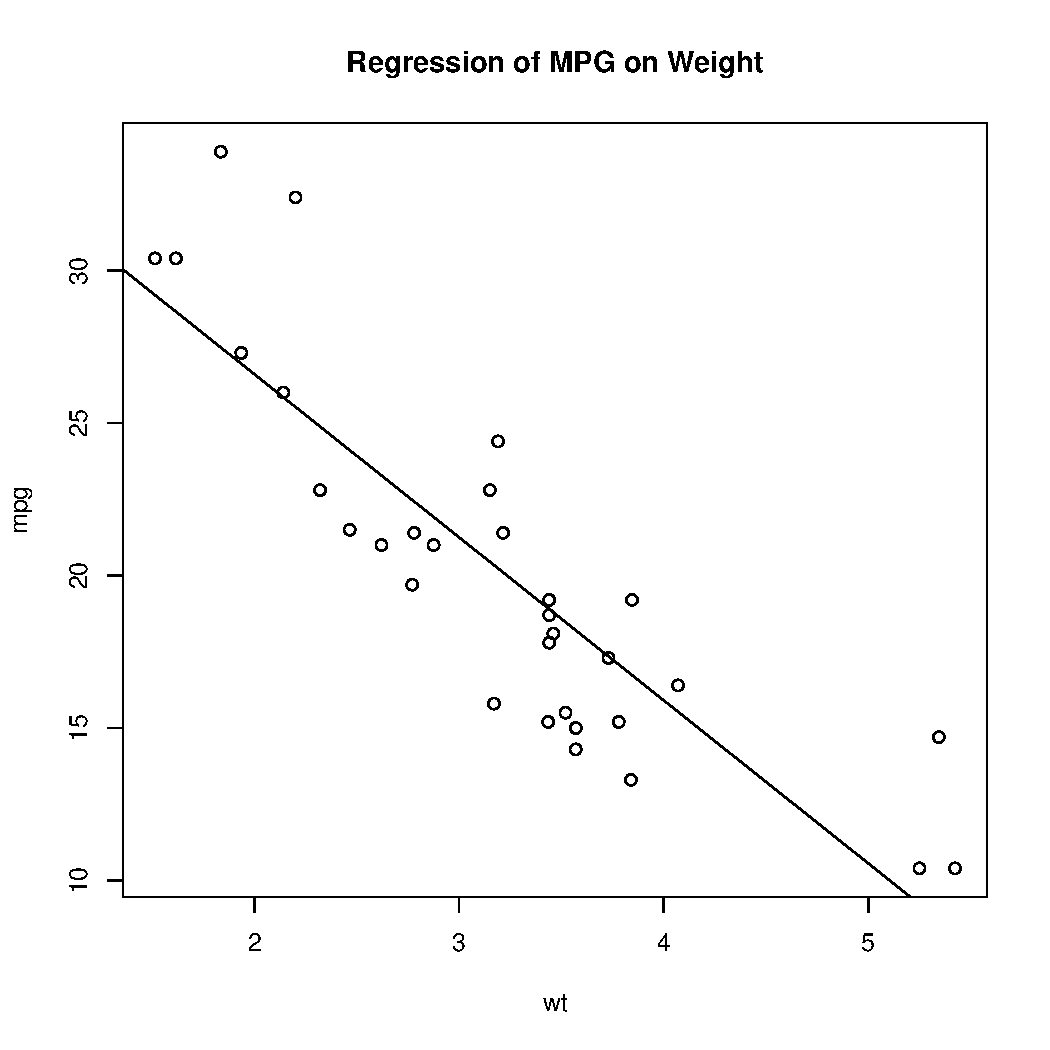
\includegraphics[width=\textwidth]{mygraph.pdf}
  \caption{first figure.}
  \label{fig:plot}
\end{figure}

\lipsum[2]

\section{Citations}
\label{sec:cite}

\citet{ananth1997regression} did something 
\lipsum[1]

A lot of work has been done \citep[e.g.,][]{ananth1997regression}.
\lipsum[2]
Some parametric bootstrap sample size approach was proposed by
\citet{hu2023hierarchical}. 
\citep{poole1971assumptions}.

\bibliography{refs}
\bibliographystyle{chicago}

\end{document}